\documentclass[11pt,letterpaper]{article}

% --- Typography & Layout ---
\usepackage[margin=1in]{geometry}
\usepackage{setspace}
\onehalfspacing
\usepackage[T1]{fontenc}
\usepackage[utf8]{inputenc}
\usepackage{microtype}
\usepackage{lmodern}

% --- Math ---
\usepackage{amsmath}

% --- Tables ---
\usepackage{booktabs}
\usepackage{graphicx}
\usepackage[font=small,labelfont=bf,tableposition=top]{caption}

% --- Colors & Links ---
\usepackage[dvipsnames]{xcolor}
\usepackage[colorlinks=true,linkcolor=MidnightBlue,citecolor=MidnightBlue,urlcolor=MidnightBlue]{hyperref}

% Renumber tables/figures with an "S" prefix for Supplementary Information
\renewcommand{\thetable}{S\arabic{table}}
\renewcommand{\thefigure}{S\arabic{figure}}

% --- Custom Math Notation (matching manuscript.tex) ---
\newcommand{\dself}{d_{\mathrm{self}}}
\newcommand{\dref}{d_{\mathrm{ref}}}

\begin{document}

\begin{center}
{\Large\bfseries Supplementary Information for:\\[0.3em] Examining the Relational Content and Personal Determinants of Social Signatures Across Multiple Time Scales}

\vspace{1.5em}
\large Omar Lizardo$^{1,\ast}$ and David Hachen$^{2}$

\vspace{1em}
\normalsize
$^{1}$Department of Sociology, University of California, Los Angeles, Los Angeles, CA, USA\\
$^{2}$Department of Sociology, University of Notre Dame, Notre Dame, IN, USA

\vspace{1em}
$^{\ast}$Corresponding author. Email: \texttt{olizardo@soc.ucla.edu}
\end{center}
\vspace{1em}

\section*{Supplementary Table S1: Per-Channel Robustness Comparison}

The main text pools all outgoing communication events (voice calls, SMS, MMS, and WhatsApp messages) into a single, equal-weighted measure of communication effort, a simplification discussed in the Limitations section. Table~\ref{tab:channel_robustness} reports the headline results separately for the voice-call channel alone, the combined text-based channels alone (SMS, MMS, and WhatsApp), and the pooled measure used in the main text, using identical semester-window definitions, eligibility criteria ($\ge 2$ alters and $>10$ channel-specific events per window), and data-quality exclusions throughout.

\begin{table}[htbp]
\centering
\caption{Per-Channel Robustness Comparison: Calls-Only vs.\ Texts-Only vs.\ Pooled (Semester Windows)}
\label{tab:channel_robustness}
\small
\resizebox{\textwidth}{!}{%
\begin{tabular}{lccc}
\toprule
\textbf{Metric} & \textbf{Calls-Only} & \textbf{Texts-Only (SMS+MMS+WhatsApp)} & \textbf{Pooled (Main Text)} \\
\midrule
Eligible Egos ($N$) & 285 & 283 & 307 \\
Mean Self-Divergence ($\dself$) & 0.062 & 0.066 & 0.066 \\
Mean Reference-Divergence ($\dref$) & 0.120 & 0.139 & 0.132 \\
Wilcoxon Signed-Rank Test ($p$, $\dself < \dref$) & $< 0.0001$ & $< 0.0001$ & $< 0.0001$ \\
Mean Power-Law Exponent ($\alpha$) & 1.18 & 1.94 & 1.94 \\
Power-Law Preferred over Exponential by AIC (\%) & 96.6\% & 38.2\% & 60.8\% \\
Rank 1 Alter is Family (\%) & 72.1\% & 19.5\% & 23.3\% \\
Rank 1 Alter is Friend (\%) & 16.0\% & 56.1\% & 53.1\% \\
Rank 1 Alter Retained Across Semesters (\%) & 59.9\% & 41.0\% & 40.5\% \\
Rank 1 Dyads Matched to Survey ($N$) & 933 & 912 & 1,003 \\
\bottomrule
\end{tabular}%
}
\end{table}

\paragraph{Interpretation.} Two conclusions follow from this comparison. First, the core persistence finding---that intraindividual self-divergence is reliably smaller than interindividual reference-divergence---is channel-invariant: it holds with $p < 0.0001$ whether the signature is built from calls alone, texts alone, or the pooled measure, confirming that signature stability is not an artifact of the equal-weighting assumption or of any single channel's measurement properties. Second, the channel-specific compositional and curvature findings reported in the main text are not channel-invariant. The voice-call channel alone shows a kinship-dominated, power-law-preferred, more stable primary slot (72.1\% family at Rank 1, 96.6\% power-law preference, 59.9\% top-alter retention). The text-based channels alone instead show a friend-dominated, more volatile primary slot with a steeper decay exponent and weaker power-law preference (19.5\% family, 56.1\% friend, 38.2\% power-law preference, 41.0\% retention). Because text messages constitute 97.7\% of all logged NetHealth communication events, the pooled measure used in the main text closely tracks the text-only channel on every metric (e.g., $\alpha = 1.94$ for both texts-only and pooled), while the comparatively rare but higher-investment voice-call channel is numerically diluted. This confirms the main text's interpretation that the friend-dominated composition documented for the pooled Rank 1 slot is substantially attributable to the equal per-event weighting of a high-volume, low-marginal-cost channel (texting) alongside a low-volume, high-investment channel (calling), rather than reflecting a difference in the underlying persistence or slot-filling mechanisms, both of which hold across all three channel definitions.

\clearpage
\section*{Supplementary Table S2: Statistical Tests of Signature Persistence}

Table~\ref{tab:supp_stability} reports the full statistical comparison between intraindividual self-divergence ($\dself$) and interindividual reference-divergence ($\dref$) across all eight temporal window schemes evaluated in the main text (Section~4.2).

\begin{table}[htbp]
\centering
\caption{Statistical Tests of Social Signature Persistence Across Window Schemes}
\label{tab:supp_stability}
\small
\resizebox{\textwidth}{!}{%
\begin{tabular}{lcccccc}
\toprule
\textbf{Scheme} & \textbf{Egos ($N$)} & \textbf{Mean $\dself$ (SD)} & \textbf{Mean $\dref$ (SD)} & \textbf{Difference} & \textbf{Wilcoxon $V$} & \textbf{$p$-value} \\
\midrule
Academic Years & 405 & 0.0584 (0.0640) & 0.1255 (0.0464) & $-0.0671$ & 7,151.0 & $< 0.0001$ \\
Semesters & 307 & 0.0658 (0.0630) & 0.1324 (0.0437) & $-0.0666$ & 3,602.0 & $< 0.0001$ \\
Quarters & 259 & 0.0425 (0.0264) & 0.1342 (0.0418) & $-0.0918$ & 0.0 & $< 0.0001$ \\
Months & 208 & 0.0414 (0.0189) & 0.1369 (0.0359) & $-0.0954$ & 0.0 & $< 0.0001$ \\
Common Cohort (Sem) & 208 & 0.0582 (0.0559) & 0.1260 (0.0439) & $-0.0678$ & 1,419.0 & $< 0.0001$ \\
Common Cohort (Mo) & 208 & 0.0414 (0.0189) & 0.1369 (0.0359) & $-0.0954$ & 0.0 & $< 0.0001$ \\
3-Week Rolling & 187 & 0.0182 (0.0077) & 0.1379 (0.0353) & $-0.1197$ & 0.0 & $< 0.0001$ \\
2-Week Discrete & 180 & 0.0450 (0.0169) & 0.1388 (0.0321) & $-0.0938$ & 0.0 & $< 0.0001$ \\
\bottomrule
\end{tabular}%
}
\end{table}

\clearpage
\section*{Supplementary Figure S1: Parameter Burn-In Convergence}

\begin{figure}[htbp]
\centering
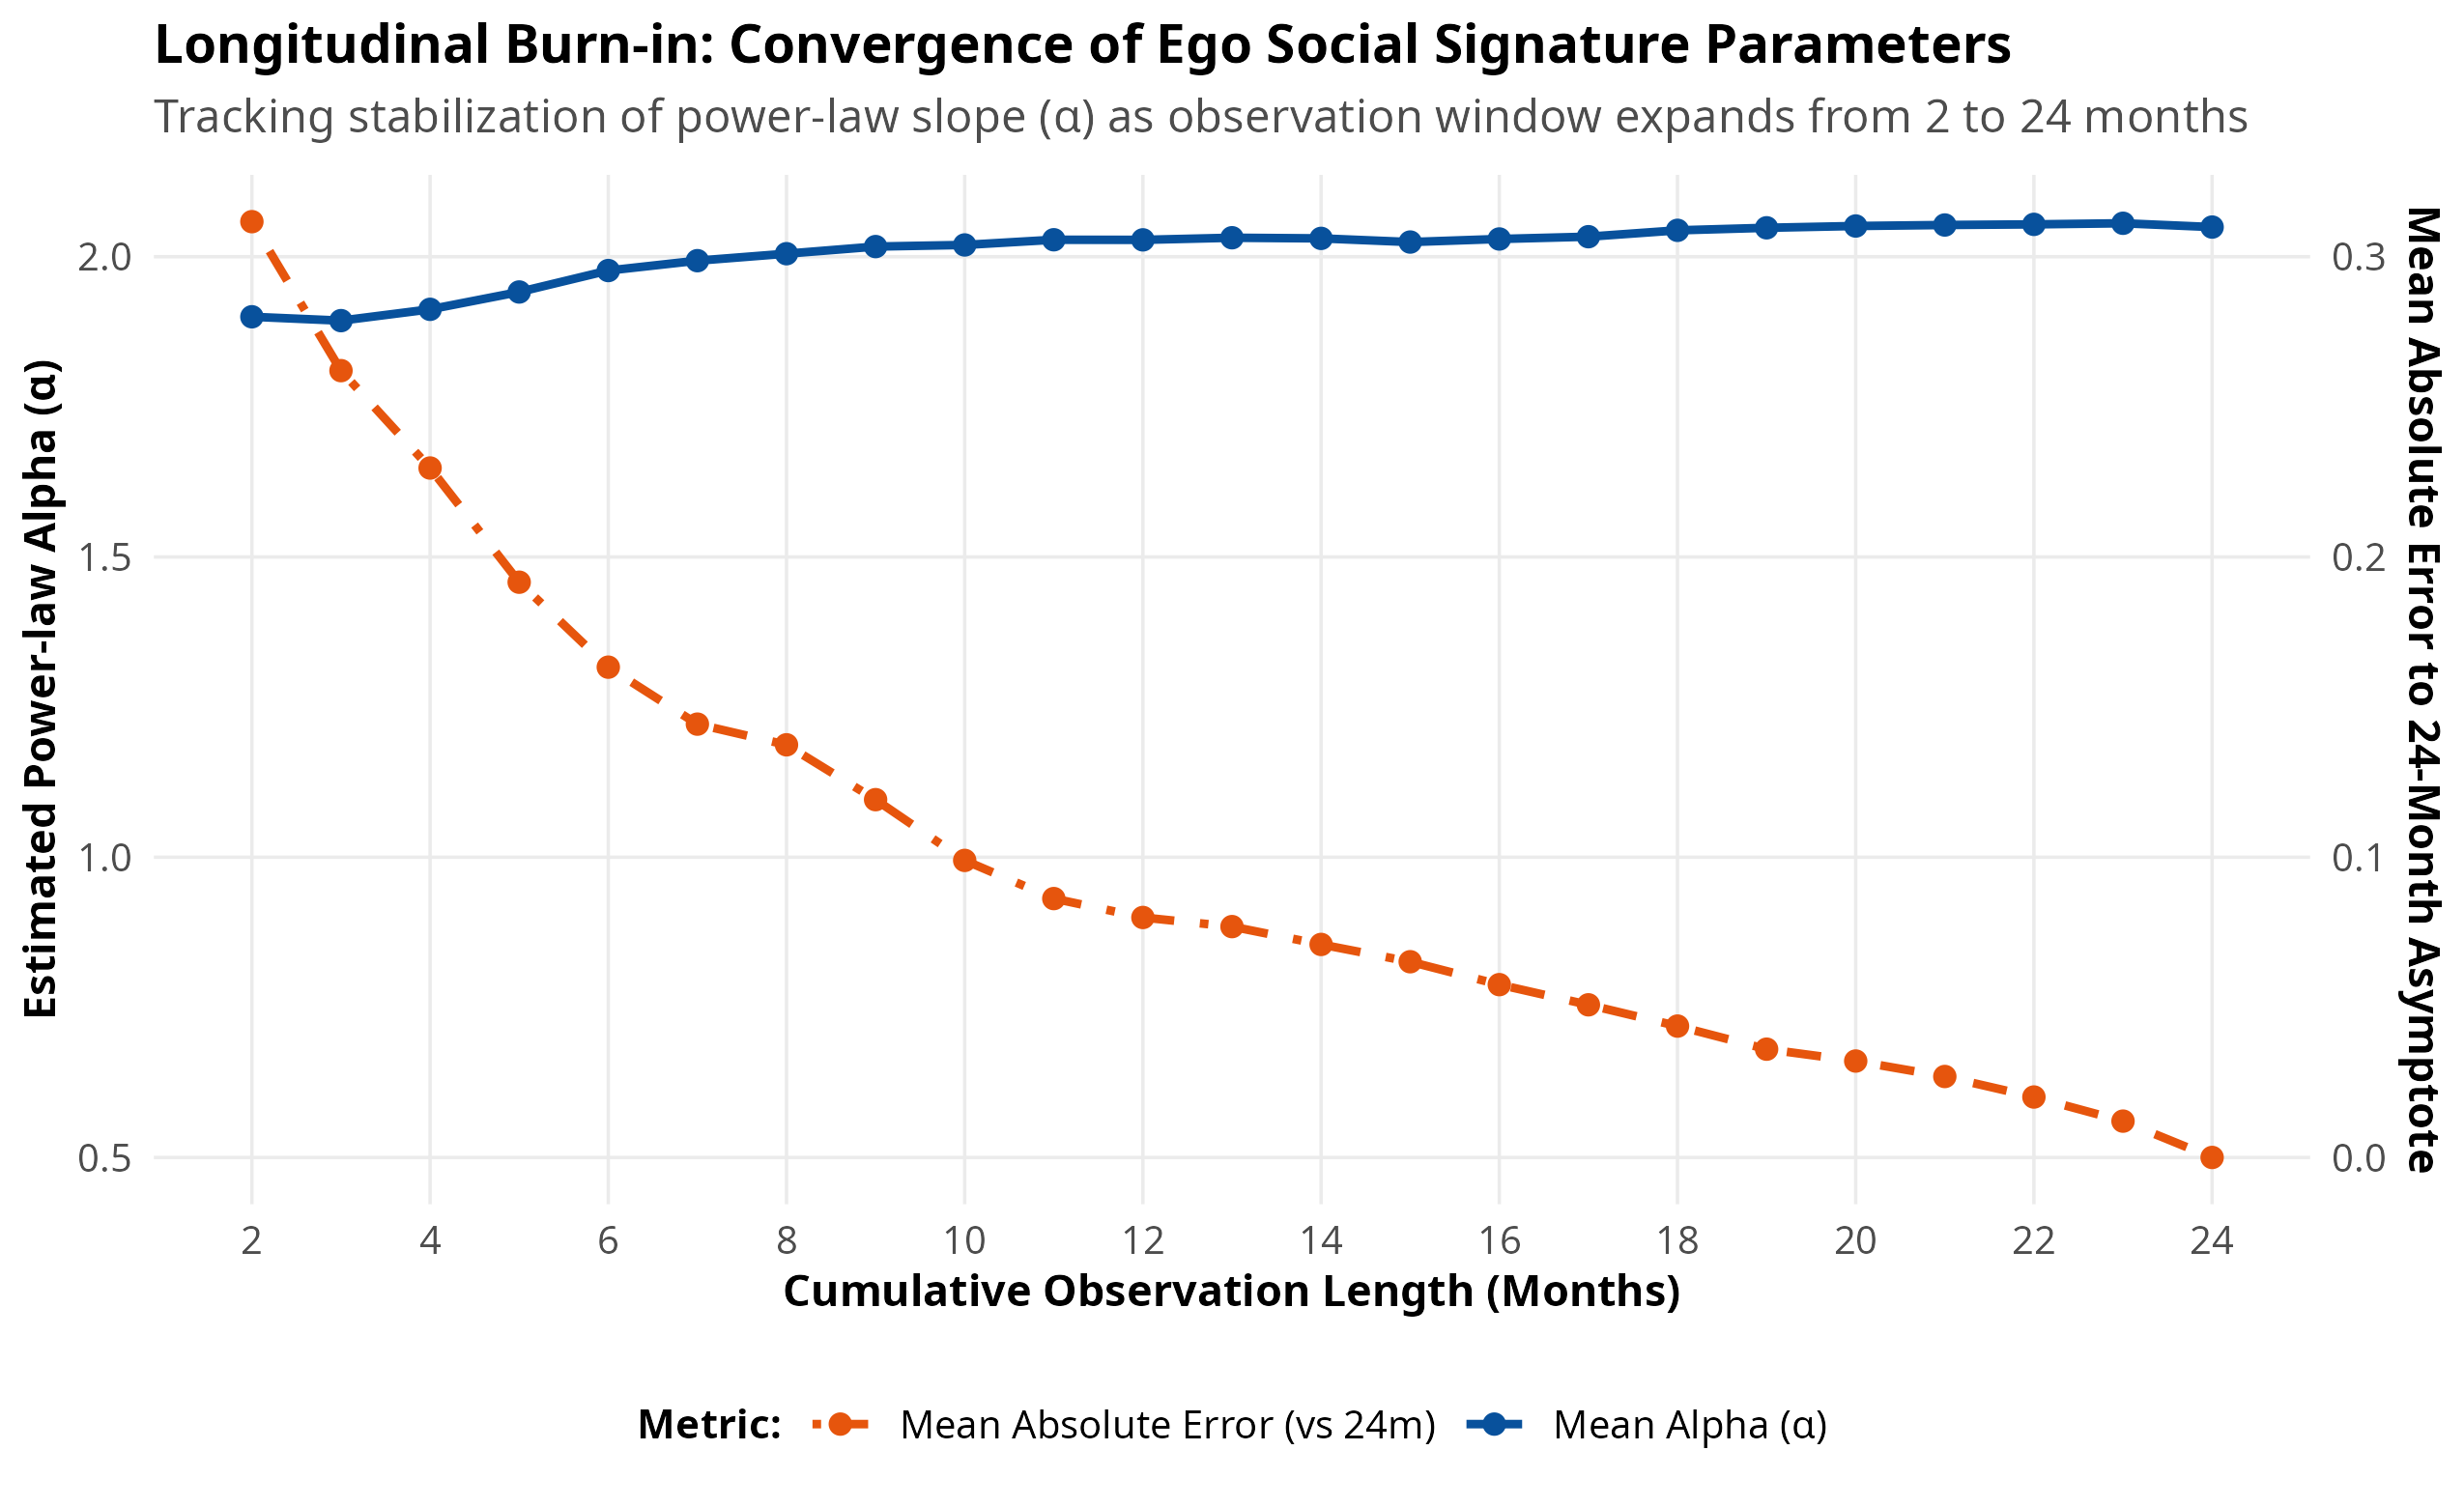
\includegraphics[width=0.9\textwidth]{Plots/fig04_parameter_burnin.png}
\caption{Parameter Burn-In Convergence Over 24 Months. Left axis shows mean estimated power-law $\alpha$; right axis shows mean absolute error relative to the 24-month asymptotic parameter value. See main text Section~4.3.}
\label{fig:supp_burnin}
\end{figure}

\clearpage
\section*{Supplementary Table S3: Parametric Model Evaluation}

Table~\ref{tab:supp_parametric} reports the full power-law versus exponential model comparison underlying the summary statistics in main text Section~4.3.

\begin{table}[htbp]
\centering
\caption{Parametric Model Evaluation Across Window Resolutions}
\label{tab:supp_parametric}
\small
\begin{tabular}{lcccccc}
\toprule
\textbf{Scheme} & \textbf{Models ($N$)} & \textbf{Power-Law $\alpha$ (SD)} & \textbf{Power-Law $R^2$} & \textbf{Exp $\beta$} & \textbf{Exp $R^2$} & \textbf{\% PL Preferred} \\
\midrule
Semesters & 1,226 & 1.94 (0.33) & 0.933 & 0.08 & 0.900 & 60.8\% \\
Months & 4,985 & 1.77 (0.43) & 0.912 & 0.19 & 0.911 & 47.8\% \\
\bottomrule
\end{tabular}
\end{table}

\clearpage
\section*{Supplementary Figure S2: Dimensions of Social Support Across Signature Rank Tiers}

\begin{figure}[htbp]
\centering
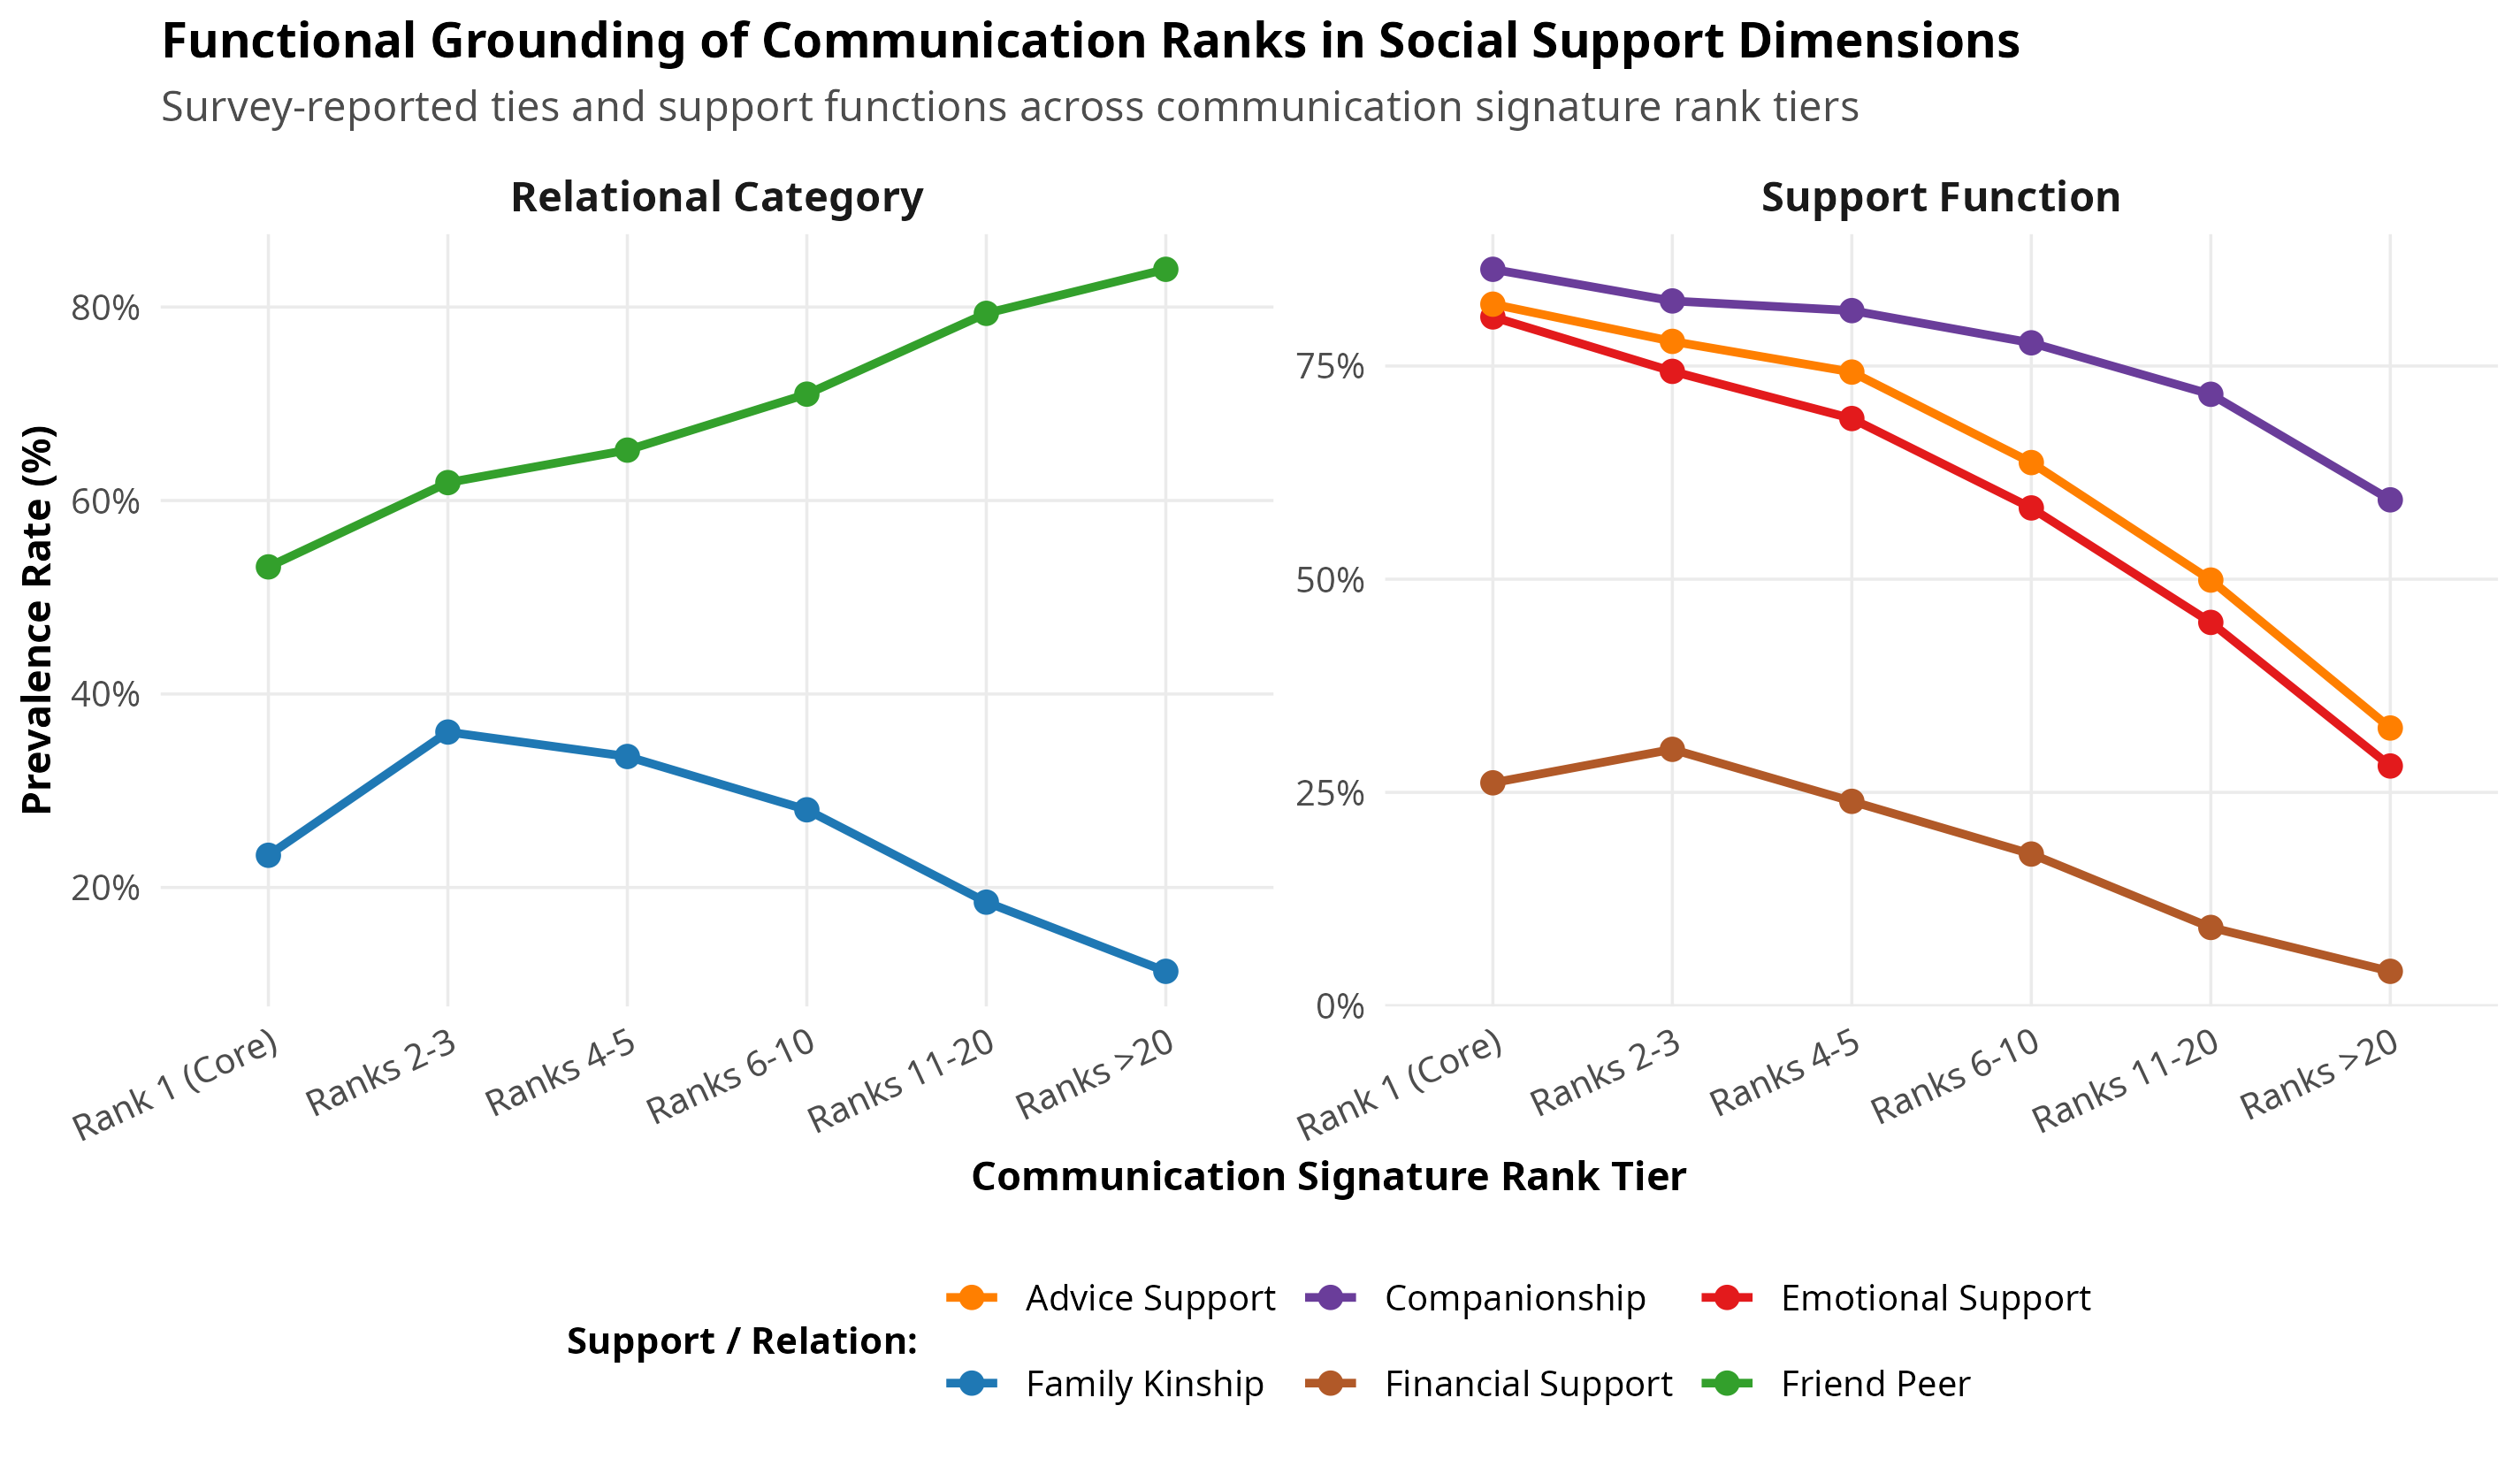
\includegraphics[width=0.95\textwidth]{Plots/fig05_rank_by_support_tiers.png}
\caption{Dimensions of Social Support Across Signature Rank Tiers. Shows prevalence rates of relational categories (left panel) and substantive social support provisions (right panel), visualizing the data reported in main text Table~2.}
\label{fig:supp_support_tiers}
\end{figure}

\clearpage
\section*{Supplementary Table S4: Tie-Attribute Regressions}

Table~\ref{tab:supp_tie_regressions} reports the full linear mixed-effects models predicting signature allocation and rank from tie attributes, underlying the summary reported in main text Section~5.2.

\begin{table}[htbp]
\centering
\caption{Linear Mixed-Effects Models Predicting Signature Allocation and Rank from Tie Attributes ($N = 16,496$ Dyad-Window Observations across 295 Egos)}
\label{tab:supp_tie_regressions}
\small
\resizebox{\textwidth}{!}{%
\begin{tabular}{lcccc}
\toprule
\textbf{Predictor Term} & \textbf{Model 1 (Evaluative)} & \textbf{Model 2 (+ Duration)} & \textbf{Model 3 (+ Salience)} & \textbf{Model 4 (Full Rank)} \\
\midrule
Intercept & $-0.124^{***}\ (0.0061)$ & $-0.143^{***}\ (0.0064)$ & $-0.160^{***}\ (0.0062)$ & $67.5^{***}\ (1.36)$ \\
Subjective Closeness (1--4) & $0.0349^{***}\ (0.0020)$ & $0.0389^{***}\ (0.0020)$ & $0.0237^{***}\ (0.0021)$ & $-6.19^{***}\ (0.45)$ \\
Interpersonal Trust (1--10) & $0.0059^{***}\ (0.0007)$ & $0.0076^{***}\ (0.0007)$ & $0.0066^{***}\ (0.0007)$ & $-0.376^{*}\ (0.15)$ \\
Tie Duration (Years) & -- & $-0.0013^{***}\ (0.0001)$ & $-0.0013^{***}\ (0.0001)$ & $-0.222^{***}\ (0.03)$ \\
Cognitive Salience ($26 - \text{Order}$) & -- & -- & $0.0038^{***}\ (0.0002)$ & $-1.09^{***}\ (0.04)$ \\
\midrule
Dependent Variable & Comm.\ Proportion ($p$) & Comm.\ Proportion ($p$) & Comm.\ Proportion ($p$) & Signature Rank ($r$) \\
Dyad-Window Observations & 16,496 & 16,496 & 16,496 & 16,496 \\
Ego Clusters & 295 & 295 & 295 & 295 \\
Ego Random Variance ($\tau_{00}$) & 0.00063 & 0.00077 & 0.00047 & 29.77 \\
Residual Variance ($\sigma^2$) & 0.00917 & 0.00908 & 0.00889 & 411.69 \\
Intraclass Correlation (ICC) & 0.065 & 0.079 & 0.051 & 0.067 \\
\bottomrule
\multicolumn{5}{l}{\footnotesize Standard errors in parentheses. $^{***}p < 0.0001$, $^{**}p < 0.01$, $^*p < 0.05$.}
\end{tabular}%
}
\end{table}

\clearpage
\section*{Supplementary Table S5: Multilevel Models of Signature Divergence}

Table~\ref{tab:supp_multilevel} reports the full multilevel linear mixed-effects models predicting signature self-divergence, underlying the summary reported in main text Section~5.3.

\begin{table}[htbp]
\centering
\caption{Multilevel Linear Mixed-Effects Models Predicting Signature Self-Divergence (JSD)}
\label{tab:supp_multilevel}
\small
\resizebox{\textwidth}{!}{%
\begin{tabular}{lccc}
\toprule
\textbf{Predictor Term} & \textbf{Model 1 (Turnover)} & \textbf{Model 2 (Topology)} & \textbf{Model 3 (Integrated)} \\
\midrule
Intercept & $-0.207^{***}\ (0.0227)$ & $-0.210^{***}\ (0.0279)$ & $-0.170^{***}\ (0.0430)$ \\
Alter Turnover ($1 - $Jaccard) & $0.371^{***}\ (0.0306)$ & $0.346^{***}\ (0.0301)$ & $0.349^{***}\ (0.0370)$ \\
\% Activity Change ($|\Delta$Events$|$/Events) & -- & $0.00027^{***}\ (0.00004)$ & $0.00020^{***}\ (0.00005)$ \\
Ego Network Clustering Coefficient & -- & $0.023\ (0.023)$ & $0.041^\dagger\ (0.023)$ \\
Ego Network Density & -- & $0.002\ (0.023)$ & -- \\
Baseline Extraversion & -- & -- & $-0.0048\ (0.0054)$ \\
Baseline Negative Emotionality & -- & -- & $-0.0180^{*}\ (0.0072)$ \\
\midrule
Observations & 921 & 915 & 642 \\
Ego Groups & 307 & 307 & 307 \\
\bottomrule
\multicolumn{4}{l}{\footnotesize Standard errors in parentheses. $^{***}p < 0.001$, $^{**}p < 0.01$, $^*p < 0.05$, $^\dagger p < 0.10$.}
\end{tabular}%
}
\end{table}

\clearpage
\section*{Supplementary Table S6: Personality Determinants of Signature Shape}

Table~\ref{tab:supp_personality} reports the full OLS regression of ego-mean power-law decay exponents on Big Five personality traits, underlying the summary reported in main text Section~5.4.

\begin{table}[htbp]
\centering
\caption{Personality Determinants of Social Signature Power-Law Alpha ($\alpha_i$)}
\label{tab:supp_personality}
\small
\begin{tabular}{lcccc}
\toprule
\textbf{Term} & \textbf{Estimate} & \textbf{Std.\ Error} & \textbf{$t$ value} & \textbf{$p$-value} \\
\midrule
(Intercept) & $1.973^{***}$ & 0.194 & 10.17 & $< 0.0001$ \\
Extraversion & $-0.026$ & 0.021 & $-1.22$ & 0.224 \\
Negative Emotionality & $0.076^{**}$ & 0.024 & 3.19 & 0.0016 \\
Agreeableness & $-0.014$ & 0.031 & $-0.44$ & 0.659 \\
Conscientiousness & $-0.003$ & 0.028 & $-0.09$ & 0.927 \\
Openness & $-0.034$ & 0.034 & $-1.01$ & 0.314 \\
Personal Network Degree & $0.0001$ & 0.003 & 0.04 & 0.969 \\
\midrule
\multicolumn{5}{l}{\footnotesize $N = 304$ egos, $R^2 = 0.058, F(6, 297) = 3.05, p = 0.0065$.}
\end{tabular}
\end{table}

\clearpage
\section*{Supplementary Figure S3: CART Decision Tree}

\begin{figure}[htbp]
\centering
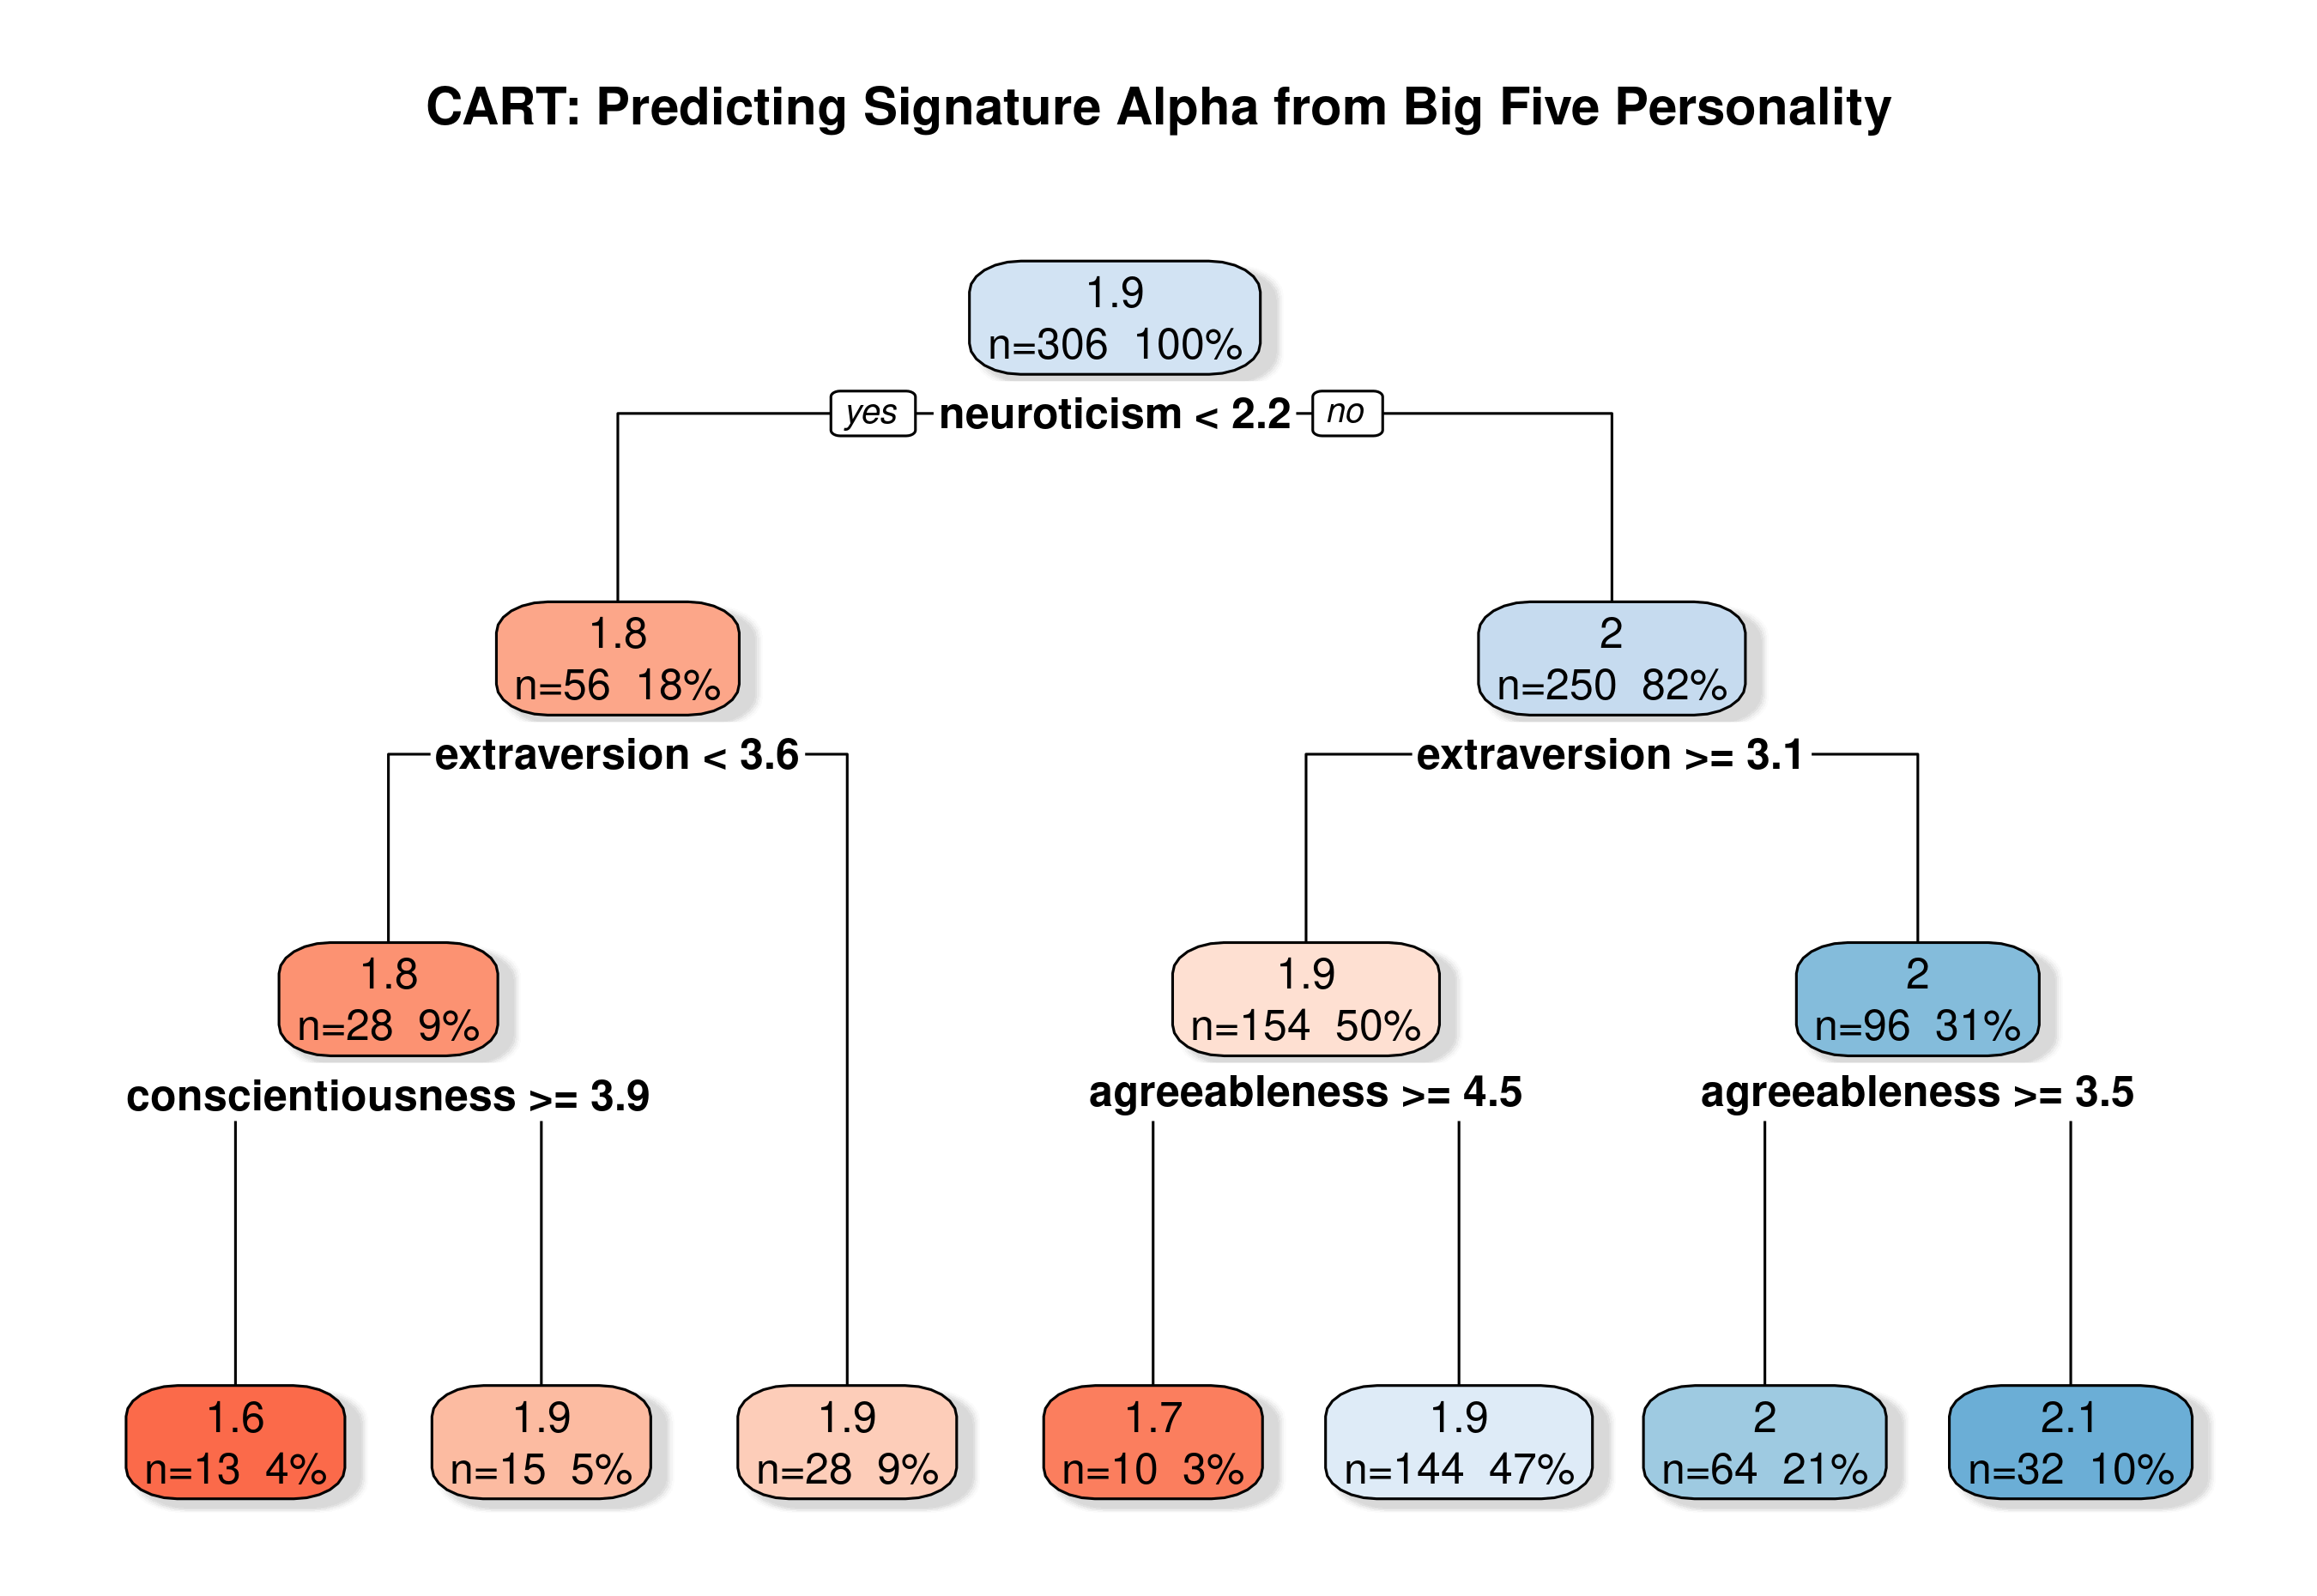
\includegraphics[width=0.95\textwidth]{Plots/fig08_cart_decision_tree.png}
\caption{Classification and Regression Tree (CART) Predicting Social Signature Power-Law Alpha ($\alpha_i$) from Big Five Personality Traits ($N = 306$). Node boxes display predicted mean $\alpha_i$ (top) and sample size (bottom). Cross-validated error exceeds 1.0 at every split, indicating weak out-of-sample predictive value; the tree is reported as an exploratory, descriptive structure only. See main text Section~5.4.}
\label{fig:supp_cart}
\end{figure}

\end{document}
